\section{Introduction}
\label{sec:intro}

Multi-criteria decision making over large databases is important in many real-world applications.
A common approach to facilitating user decision-making in databases is to model user preference as a \textit{utility function} \cite{CB00, NL12, NS10}, which assigns each tuple a numerical score. Knowledge of this function—either explicit or implicit—enables systems to reduce user effort in identifying preferred tuples. Two major paradigms built on this assumption are (1) the \emph{top-$k$ query} \cite{GY05, PL07, SI07, LYH09, LC09} and (2) the \emph{skyline query} \cite{CJ06, CJ062, LY07, MC09, PT05}.
(1) In a top-$k$ query, the user explicitly provides a utility function and an integer $k$, and the system returns the $k$ highest-scoring tuples. While conceptually straightforward, this approach is impractical when the user cannot specify precise weights in the utility function—especially in high-dimensional data, where hundreds of attributes make this specification infeasible.
(2) The skyline query, by contrast, assumes only that the utility function is component-wise monotonic: if one tuple is no worse than another in every attribute, its utility is at least as high. The system thus returns all skyline points, i.e., tuples not dominated by any other. Although this avoids explicit utility specification, the output can become unmanageably large. As dimensionality increases, domination becomes less common and the skyline typically contains more tuples, potentially overwhelming the user.

Recently, the $k$-regret query~\cite{AK17, asudeh2017efficient, NS10, PW14, XW18} has emerged as a promising solution to the limitations of top-$k$ and skyline queries. The method selects $k$ representative tuples such that, for any possible user preference, the best tuple in the returned set closely approximates the global optimum in the database. The regret ratio measures the relative utility loss incurred by choosing from the returned set rather than the entire database (Section~\ref{sec:def}). The objective is to minimize the maximum regret ratio over the admissible utility functions.

These frameworks operate in a single round, presenting their results at once. This naturally raises the question: can multiple rounds of interaction further reduce regret or output size? To address this, interactive regret minimization frameworks~\cite{NL12, XCL19} have been proposed, where the system iteratively presents a few candidate tuples per round, learns the user’s implicit utility function from their choices, and progressively refines subsequent recommendations.

Most previous studies have focused on databases with a small number of attributes, typically 2-10, and often require users to specify their attributes of interest beforehand. In contrast, this paper considers a \textit{high-dimensional setting} with more than a hundred attributes and no prior attribute selection. These scenarios are increasingly common nowadays, e.g., in housing markets (price, size, location, etc.) and financial products (interest rate, liquidity, historical performance, etc.). In these domains, the high dimensionality poses significant challenges: computational costs grow exponentially, theoretical guarantees become weaker, and traditional algorithms often fail to provide meaningful representative subsets. There is an urgent need for efficient and effective algorithms that address these challenges.

We want algorithms that satisfy the following requirements:

\begin{itemize}[beginpenalty=10000]
    \item \textit{Quality.} Return a small, manageable set with low regret, ideally identifying the user’s favorite tuple in the database.
    
    \item \textit{Efficiency.} Execute within a reasonable time on high-dimensional datasets that may contain millions of tuples.
    
    \item \textit{Usability.} Require few interactions, using simple, intuitive questions that remain manageable as dimensionality grows.
\end{itemize}

Our work is motivated by the observation that users typically base decisions on a small subset of salient attributes rather than the full feature set. For example, a house may be described by hundreds of attributes, including floor area, nearby amenities, and energy efficiency, yet buyers often focus primarily on a few factors such as price, size, and location. This behavior is well documented in cognitive psychology~\cite{GG96, GA12, MH99, GG99} and conjoint analysis~\cite{WX22, SC05, TK03, DMW12}, and is further supported by our survey.

In psychology, the “Take-The-Best” heuristic~\cite{GG96, GA12} shows that people make accurate decisions using only a few salient attributes. It ranks attributes by importance and bases each choice on the first attributes that distinguish the alternatives, ignoring the rest. Despite its simplicity, it can outperform more complex models, including multiple regression and weighted integration~\cite{MH99, GG99}. This finding supports our high-dimensional $k$-regret setting and motivates the assumption that the true utility vector is sparse, with most weight concentrated on a small subset of attributes.

Conjoint analysis similarly estimates preferences over multiple attributes from evaluations or choices among alternatives~\cite{WX22, SC05, TK03, DMW12}. Estimated attribute contributions yield relative importance scores, providing evidence that importance can be concentrated on a small subset of attributes. In Schaupp and Bélanger's study, the five highest-ranked attributes account for $84.2\%$ of the reported relative importance~\cite{SC05}. This concentration of importance motivates our sparse-utility model.

To examine how many attributes users consider in decision making, we surveyed $30$ participants using the Car, House, and NBA datasets described in Section~\ref{sec:eval}. Participants were shown a set of options and asked to identify the attributes they considered when comparing them. They could select any number of attributes, with no minimum or maximum imposed. The datasets contain $57$, $33$, and $104$ attributes, respectively. Figure~\ref{fig:num_att} summarizes the number of attributes selected for each dataset and shows that most participants relied on only a small subset. For the Car dataset, $12$ participants ($40\%$) considered exactly $3$ of the $57$ attributes, with \textit{Real-World MPG}, \textit{Model Year}, and \textit{Engine Displacement} being the three most frequently selected. Across all datasets, more than $80\%$ of participants considered at most $5$ attributes. These results provide empirical support for our assumption that users' effective utility functions are sparse.

\begin{figure}[h]
    \centering
    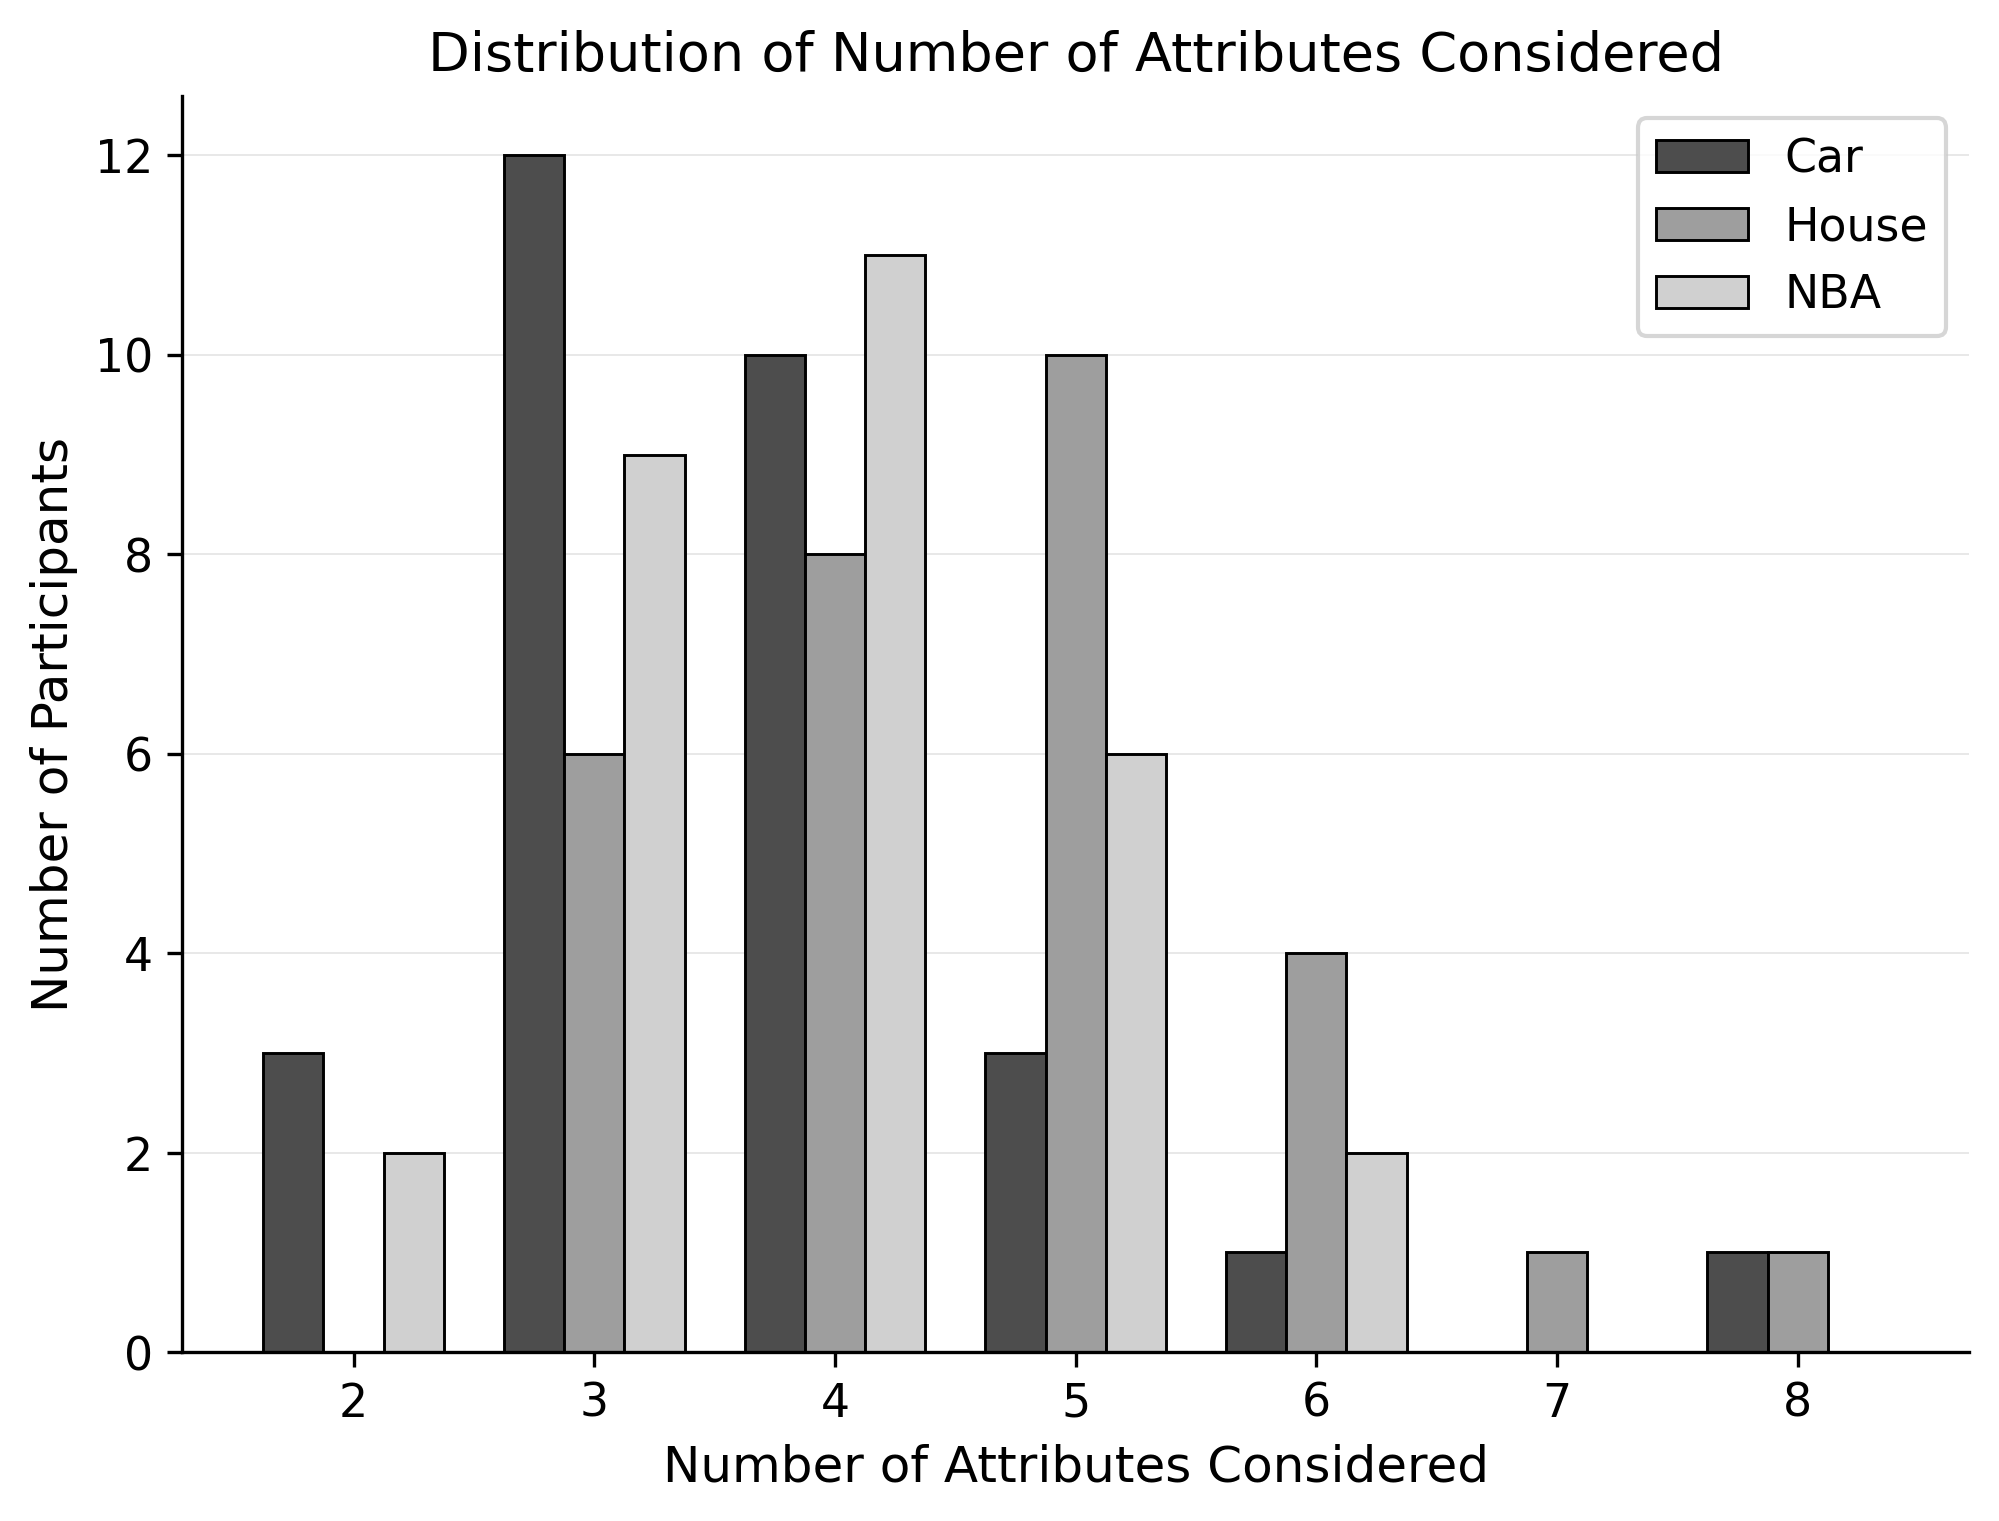
\includegraphics[width=0.7\linewidth]{plot/num_att.png}
    \caption{Survey on Number of Attributes Considered}
    \label{fig:num_att}
\end{figure}

Motivated by this, we introduce FHDR (\underline{F}ast \underline{H}igh-\underline{D}imensional \underline{R}eduction), a generic framework for $k$-regret minimization in high-dimensional settings. Our major contributions are as follows:
\begin{itemize}
    \item We present FHDR, a framework for high-dimensional regret minimization under sparse linear preferences. It handles datasets of arbitrary original dimensionality and identifies the user's favorite tuple with sufficient feedback, requiring substantially fewer questions in the evaluated comparisons.
    \item We implicitly discover the user's key attributes through tuple comparisons, avoiding upfront attribute selection requirement in previous papers.
    \item We support flexible interaction, including zero feedback. The user can skip or stop answering questions at any time, ensuring a user-friendly interaction process.
    \item We propose a single-round algorithm \textsc{AttributeSubset} for any dimensionality, which is more than $10$ times faster than existing single-round algorithms under high-dimensional settings.
    \item We conduct extensive experiments on synthetic and real datasets to evaluate regret ratio, computation time, and interaction cost. A user study on Car further evaluates FHDR's end-to-end recommendation quality and usability.
\end{itemize}

The rest of the paper is organized as follows: Section~\ref{sec:related} discusses related work, and Section~\ref{sec:def} gives the problem definition. The complete algorithm for high-dimensional regret minimization is presented in Section~\ref{sec:alg}, while the solution for limited user feedback is given in Section~\ref{sec:attsub}. Section~\ref{sec:eval} shows the experiment results and Section~\ref{sec:concl} concludes the paper.

